\documentclass[11pt]{article}
\usepackage[margin=0.85in]{geometry}
\usepackage{amsmath,amssymb,booktabs,graphicx,tikz}
\usepackage[hidelinks]{hyperref}
\usetikzlibrary{arrows.meta}
\setlength{\parindent}{0pt}
\setlength{\parskip}{7pt}
\newcommand{\parttitle}[1]{\par\textbf{#1}\par}
\begin{document}
\begin{center}
{\LARGE CIS 5190: Homework 3}\\[5pt]
{\large Written Answers}
\end{center}

\section*{Use of AI Tools}
I used AI for concepts learning as well as answer checks. I also used it to transform my written answer to Latex format.
Specifically, I used OpenAI Codex, which also generated a draft of the solutions and figures in this document.
The explanations can help me follow the steps, but I still need to check the reasoning myself so that I do not skip understanding the material.

\section*{Time Spent}
The following are AI-suggested estimates, not measured times. They should be checked against my actual time before submission.
\begin{center}
\begin{tabular}{lc}
\toprule
Part & Estimated hours \\
\midrule
Reading the assignment & 0.25 \\
Question 1 & 0.50 \\
Question 2 & 0.50 \\
Question 3 & 0.75 \\
Question 4 & 0.25 \\
Question 5 & 0.50 \\
\midrule
Total & 2.75 \\
\bottomrule
\end{tabular}
\end{center}

\newpage
\section*{Question 1: K-means}
\parttitle{(a) Two iterations}
For a point $(x,y)$ and centroid $(a,b)$, the Euclidean distance is
\[
 d=\sqrt{(x-a)^2+(y-b)^2}.
\]
We assign each point to its nearest centroid, then average the points in each cluster.

\textbf{Iteration 1.} Start with $\mu_1=(6,9)$ and $\mu_2=(8,4)$.
\begin{center}
\begin{tabular}{cccc}
\toprule
Sample & $d(S,1)$ & $d(S,2)$ & Assigned cluster \\
\midrule
$A=(2,3)$ & $\sqrt{52}=2\sqrt{13}$ & $\sqrt{37}$ & 2 \\
$B=(4,6)$ & $\sqrt{13}$ & $\sqrt{20}=2\sqrt{5}$ & 1 \\
$C=(5,1)$ & $\sqrt{65}$ & $\sqrt{10}$ & 2 \\
$D=(10,12)$ & $\sqrt{25}=5$ & $\sqrt{68}=2\sqrt{17}$ & 1 \\
\bottomrule
\end{tabular}
\end{center}
The new clusters and centroids are
\begin{align*}
 C_1&=\{B,D\}, & \mu_1&=\left(\frac{4+10}{2},\frac{6+12}{2}\right)=(7,9),\\
 C_2&=\{A,C\}, & \mu_2&=\left(\frac{2+5}{2},\frac{3+1}{2}\right)=\left(\frac72,2\right).
\end{align*}

\textbf{Iteration 2.} Now use $\mu_1=(7,9)$ and $\mu_2=(7/2,2)$.
\begin{center}
\begin{tabular}{cccc}
\toprule
Sample & $d(S,1)$ & $d(S,2)$ & Assigned cluster \\
\midrule
$A$ & $\sqrt{61}$ & $\sqrt{13}/2$ & 2 \\
$B$ & $\sqrt{18}=3\sqrt{2}$ & $\sqrt{65}/2$ & 2 \\
$C$ & $\sqrt{73}$ & $\sqrt{13}/2$ & 2 \\
$D$ & $\sqrt{18}=3\sqrt{2}$ & $\sqrt{569}/2$ & 1 \\
\bottomrule
\end{tabular}
\end{center}
The new clusters and centroids are
\begin{align*}
 C_1&=\{D\}, & \mu_1&=(10,12),\\
 C_2&=\{A,B,C\}, & \mu_2&=\left(\frac{2+4+5}{3},\frac{3+6+1}{3}\right)
 =\left(\frac{11}{3},\frac{10}{3}\right).
\end{align*}

\parttitle{(b) Four clusters}
The four centroids are $\boxed{(2,3),\ (4,6),\ (5,1),\ (10,12)}$, in any order.
Each point has its own centroid, so the total squared distance is zero. This is the global minimum because a squared distance cannot be negative.

\newpage
\section*{Question 2: PCA}
\parttitle{(a) Principal-component directions}
Both principal-component lines pass through the overall data mean. PC1 follows the direction with the largest spread, and PC2 is perpendicular to PC1. The colors do not define separate PCA problems.

\begin{center}
\begin{tabular}{@{}cc@{}}
\textbf{Original plot from the assignment} & \textbf{Same plot with PCA directions} \\[5pt]
\includegraphics[draft=false,page=3,trim=72bp 444.089bp 329.4bp 210.601bp,clip,width=7cm]{hw3.pdf}
&
\begin{tikzpicture}[baseline=0pt]
\node[anchor=south west,inner sep=0] at (0,0)
 {\includegraphics[draft=false,page=3,trim=72bp 444.089bp 329.4bp 210.601bp,clip,width=7cm]{hw3.pdf}};
\draw[red!80!black,line width=1.1pt,{Latex}-{Latex}] (0.95,2.44)--(6.5,2.44);
\node[fill=white,inner sep=2pt,text=red!80!black] at (5.8,2.74) {PC1};
\draw[black,dashed,line width=1.1pt,{Latex}-{Latex}] (3.71,0.65)--(3.71,4.08);
\node[fill=white,inner sep=2pt] at (4.2,3.8) {PC2};
\end{tikzpicture}
\\[12pt]
\includegraphics[draft=false,page=3,trim=329.401bp 442.474bp 72.001bp 208.987bp,clip,width=7cm]{hw3.pdf}
&
\begin{tikzpicture}[baseline=0pt]
\node[anchor=south west,inner sep=0] at (0,0)
 {\includegraphics[draft=false,page=3,trim=329.401bp 442.474bp 72.001bp 208.987bp,clip,width=7cm]{hw3.pdf}};
% Directions chosen visually; no PCA fit was used.
\draw[red!80!black,line width=1.1pt,{Latex}-{Latex}] (1.0,1.89)--(6.4,3.34);
\node[fill=white,inner sep=2pt,text=red!80!black] at (5.7,3.65) {PC1};
\draw[black,dashed,line width=1.1pt,{Latex}-{Latex}] (4.39,0.60)--(3.39,4.33);
\node[fill=white,inner sep=2pt] at (2.9,4.0) {PC2};
\end{tikzpicture}
\end{tabular}

\small Red solid line: PC1. Black dashed line: PC2.
The lines cross at the approximate overall mean.
\end{center}
\textbf{Left:} The greatest spread is between the two groups, so PC1 is approximately horizontal and PC2 is approximately vertical.

\textbf{Right:} Looking at all points together, the spread is mostly horizontal with a small upward tilt. PC1 therefore has a shallow positive slope, and PC2 has a steep negative slope. These are visual estimates; the exact angles cannot be read from the plot. Reversing either direction gives the same principal component.

\parttitle{(b) Retaining at least 75\% of the variance}
The total variance is
\[
2.1+1.8+1.3+0.9+0.4+0.2+0.15+0.02+0.001=6.871.
\]
The required amount is $0.75(6.871)=5.15325$.
The first two eigenvalues sum to $3.9<5.15325$, while the first three sum to
$5.2>5.15325$. Therefore, $\boxed{K=3}$, retaining approximately $75.68\%$ of the variance.

\newpage
\section*{Question 3: PCA by Hand}
\parttitle{(a) Unit-vector principal components}
The mean is
\[
\bar{x}=\left(\frac{4+2+5+1}{4},\frac{1+3+4+0}{4}\right)=(3,2).
\]
Subtract the mean from each row:
\[
Z=\begin{bmatrix}1&-1\\-1&1\\2&2\\-2&-2\end{bmatrix}.
\]
Using the covariance convention $\Sigma=Z^\top Z/4$,
\[
\Sigma=\frac14\begin{bmatrix}10&6\\6&10\end{bmatrix}
=\begin{bmatrix}5/2&3/2\\3/2&5/2\end{bmatrix}.
\]
Its eigenvalues satisfy
\[
\det(\Sigma-\lambda I)
=\left(\frac52-\lambda\right)^2-\left(\frac32\right)^2
=(\lambda-4)(\lambda-1)=0.
\]
For $\lambda_1=4$, the eigenvector satisfies $v_x=v_y$.
For $\lambda_2=1$, it satisfies $v_x=-v_y$. Normalizing gives
\[
\boxed{v_1=\frac1{\sqrt2}\begin{bmatrix}1\\1\end{bmatrix}},\qquad
\boxed{v_2=\frac1{\sqrt2}\begin{bmatrix}1\\-1\end{bmatrix}}.
\]
Bob should use $v_1$, since it retains the largest variance: $4/(4+1)=80\%$.
Using $1/(n-1)$ instead of $1/n$ changes the eigenvalues but not these directions or the retained fraction.

\parttitle{(b) Centered projections}
For each point, its one-dimensional coordinate is
$t=v_1^\top(x-\bar{x})$, and its projected point on the original plot is
$\hat{x}=\bar{x}+tv_1$. The PC1 line passes through $(3,2)$ and has equation $y=x-1$.
\begin{center}
\begin{tabular}{cccc}
\toprule
Point & Centered point & Coordinate $t$ & Projected point $\hat{x}$ \\
\midrule
$A=(4,1)$ & $(1,-1)$ & $0$ & $(3,2)$ \\
$B=(5,4)$ & $(2,2)$ & $2\sqrt2$ & $(5,4)$ \\
$C=(2,3)$ & $(-1,1)$ & $0$ & $(3,2)$ \\
$D=(1,0)$ & $(-2,-2)$ & $-2\sqrt2$ & $(1,0)$ \\
\bottomrule
\end{tabular}
\end{center}
In the original matrix row order, Bob sends $\boxed{(0,\ 0,\ 2\sqrt2,\ -2\sqrt2)}$.

\begin{center}
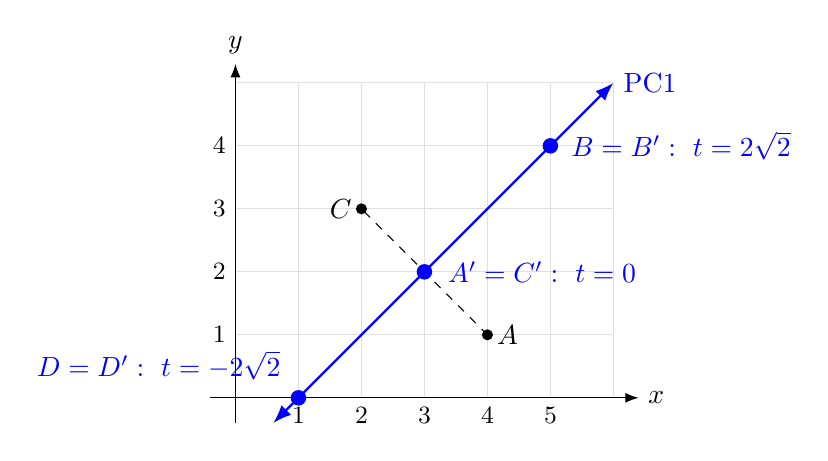
\begin{tikzpicture}[x=0.8cm,y=0.8cm]
\draw[step=1,gray!25,thin] (0,0) grid (6,5);
\draw[-{Latex}] (0,-0.4)--(0,5.3) node[above] {$y$};
\draw[-{Latex}] (-0.4,0)--(6.4,0) node[right] {$x$};
\foreach \i in {1,...,5} {\node[below] at (\i,0) {\small\i};}
\foreach \i in {1,...,4} {\node[left] at (0,\i) {\small\i};}
\draw[blue,thick,{Latex}-{Latex}] (0.6,-0.4)--(6,5) node[right] {PC1};
\draw[dashed] (4,1)--(3,2)--(2,3);
\fill (4,1) circle (2pt) node[right] {$A$};
\fill (2,3) circle (2pt) node[left] {$C$};
\fill[blue] (3,2) circle (2.8pt) node[right=5pt] {$A'=C':\ t=0$};
\fill[blue] (5,4) circle (2.8pt) node[right=4pt] {$B=B':\ t=2\sqrt2$};
\fill[blue] (1,0) circle (2.8pt) node[above left=3pt] {$D=D':\ t=-2\sqrt2$};
\end{tikzpicture}
\end{center}

\newpage
\section*{Question 4: Image Filtering / Convolution}
\parttitle{(a) Mean filter: image B}
\[
\frac19\begin{bmatrix}1&1&1\\1&1&1\\1&1&1\end{bmatrix}
\]
Each output pixel is the average of a $3\times3$ neighborhood. Averaging smooths small details and blurs the image, so the answer is $\boxed{\text{B}}$.

\parttitle{(b) Doubling pixel values: image A}
\[
\begin{bmatrix}0&0&0\\0&2&0\\0&0&0\end{bmatrix}
\]
The displayed output is $\min(2p,1)$ for an original pixel value $p\in[0,1]$.
This brightens the image and clips values of at least $0.5$ to white, so the answer is $\boxed{\text{A}}$.

\parttitle{(c) Horizontal intensity differences: image C}
\[
\begin{bmatrix}1&0&-1\\2&0&-2\\1&0&-1\end{bmatrix}
\]
This filter compares the left and right sides of a neighborhood, so it detects changes across the horizontal direction and emphasizes vertical edges. Image $\boxed{\text{C}}$ shows those edges, including the vertical tree trunks.

\newpage
\section*{Question 5: CNN Dimensions and Parameters}
For a convolution or pooling layer, each spatial output size is
\[
 n_{\mathrm{out}}=\left\lfloor\frac{n_{\mathrm{in}}+2p-k}{s}\right\rfloor+1.
\]
The padding preserves the height and width in each convolution.
Each pooling layer halves both dimensions, and ReLU does not change the shape.

\begin{center}
\begin{tabular}{lc}
\toprule
Layer & Output shape (height $\times$ width $\times$ channels) \\
\midrule
Input & $320\times320\times3$ \\
Convolution 1 + ReLU & $320\times320\times16$ \\
Max pooling 1 & $160\times160\times16$ \\
Convolution 2 + ReLU & $160\times160\times8$ \\
Max pooling 2 & $80\times80\times8$ \\
Convolution 3 + ReLU & $80\times80\times4$ \\
Max pooling 3 & $40\times40\times4$ \\
\bottomrule
\end{tabular}
\end{center}

\parttitle{(a) Output height}
$\boxed{40}$ pixels, since $320/2^3=40$.

\parttitle{(b) Output width}
$\boxed{40}$ pixels, by the same calculation.

\parttitle{(c) Output channels}
$\boxed{4}$, the number of output channels in the last convolution.

\parttitle{(d) Learnable parameters}
For a convolutional layer, the count is
\[
(k^2 C_{\mathrm{in}}+1)C_{\mathrm{out}}.
\]
Each output channel has $k^2 C_{\mathrm{in}}$ weights and one bias.
\begin{align*}
\text{Convolution 1:}&\quad (5\cdot5\cdot3+1)\cdot16=1216,\\
\text{Convolution 2:}&\quad (3\cdot3\cdot16+1)\cdot8=1160,\\
\text{Convolution 3:}&\quad (3\cdot3\cdot8+1)\cdot4=292.
\end{align*}
ReLU and max pooling have no learnable parameters, so the total is
\[
\boxed{1216+1160+292=2668}.
\]
\end{document}
